\documentclass[10pt]{article}

\usepackage{mathtools, amssymb, bm}
\usepackage{microtype}
\usepackage[utf8]{inputenc}
\usepackage[margin = 1in]{geometry}
\usepackage{booktabs}
\usepackage{graphicx}
\usepackage{xcolor}
\usepackage{tikzsymbols}
\usepackage[hidelinks]{hyperref}
\usepackage{titlesec}



% \titleformat{\section}{\normalsize\bfseries}{\thesection}{1em}{}
\titleformat{\section}{\large\bfseries}{\thesection}{1em}{}
\setcounter{secnumdepth}{0}

\definecolor{colabcol}{HTML}{960018}
\newcommand{\mycolab}[1]{\textcolor{colabcol}{\textsl{Collaborators:}} #1 \\ }
\newcommand{\mycolaba}[1]{\textcolor{colabcol}{\textsl{Collaborators:}} #1}

\title{
    {\Large Homework 5}
}
\author{
    {\normalsize Aiden Kenny}\\
    {\normalsize STAT GR5205: Linear Regression Models}\\
    {\normalsize Columbia University}
}
\date{\normalsize Novermber 25, 2020}

\begin{document}

\maketitle

\newcommand{\myg}{\mathbf{g}_{\lambda}}
\newcommand{\mygfull}{\mathbf{g}_{\lambda}(\mathbf{y})}
%' ============================================================================================================================================================
\section{Question 1} \noindent
\mycolaba{None}
\begin{itemize}
    \item[(a)] Let \(Y\) be the number of nurses in the hospital and let \(X\) be the available faculty and services. 
    The left and middle panels of Figure \ref{q01-investigation} show the histograms of \(Y\) and \(X\), respectively. We see that \(Y\) is skewed right, while 
    \(X\) appears to be normally-distributed. In addition, the scatterplot of \(Y\) vs. \(X\), which is in the third panel of Figure 
    \ref{q01-investigation}, shows that there is a nonlinear relationship between \(Y\) and \(X\). 
    All of these indicate that \(Y\) is suitable for a data transformation. Specifically, we would like to perform a 
    power transformation on \(Y\). 
    \begin{figure}[ht]
        \centering
        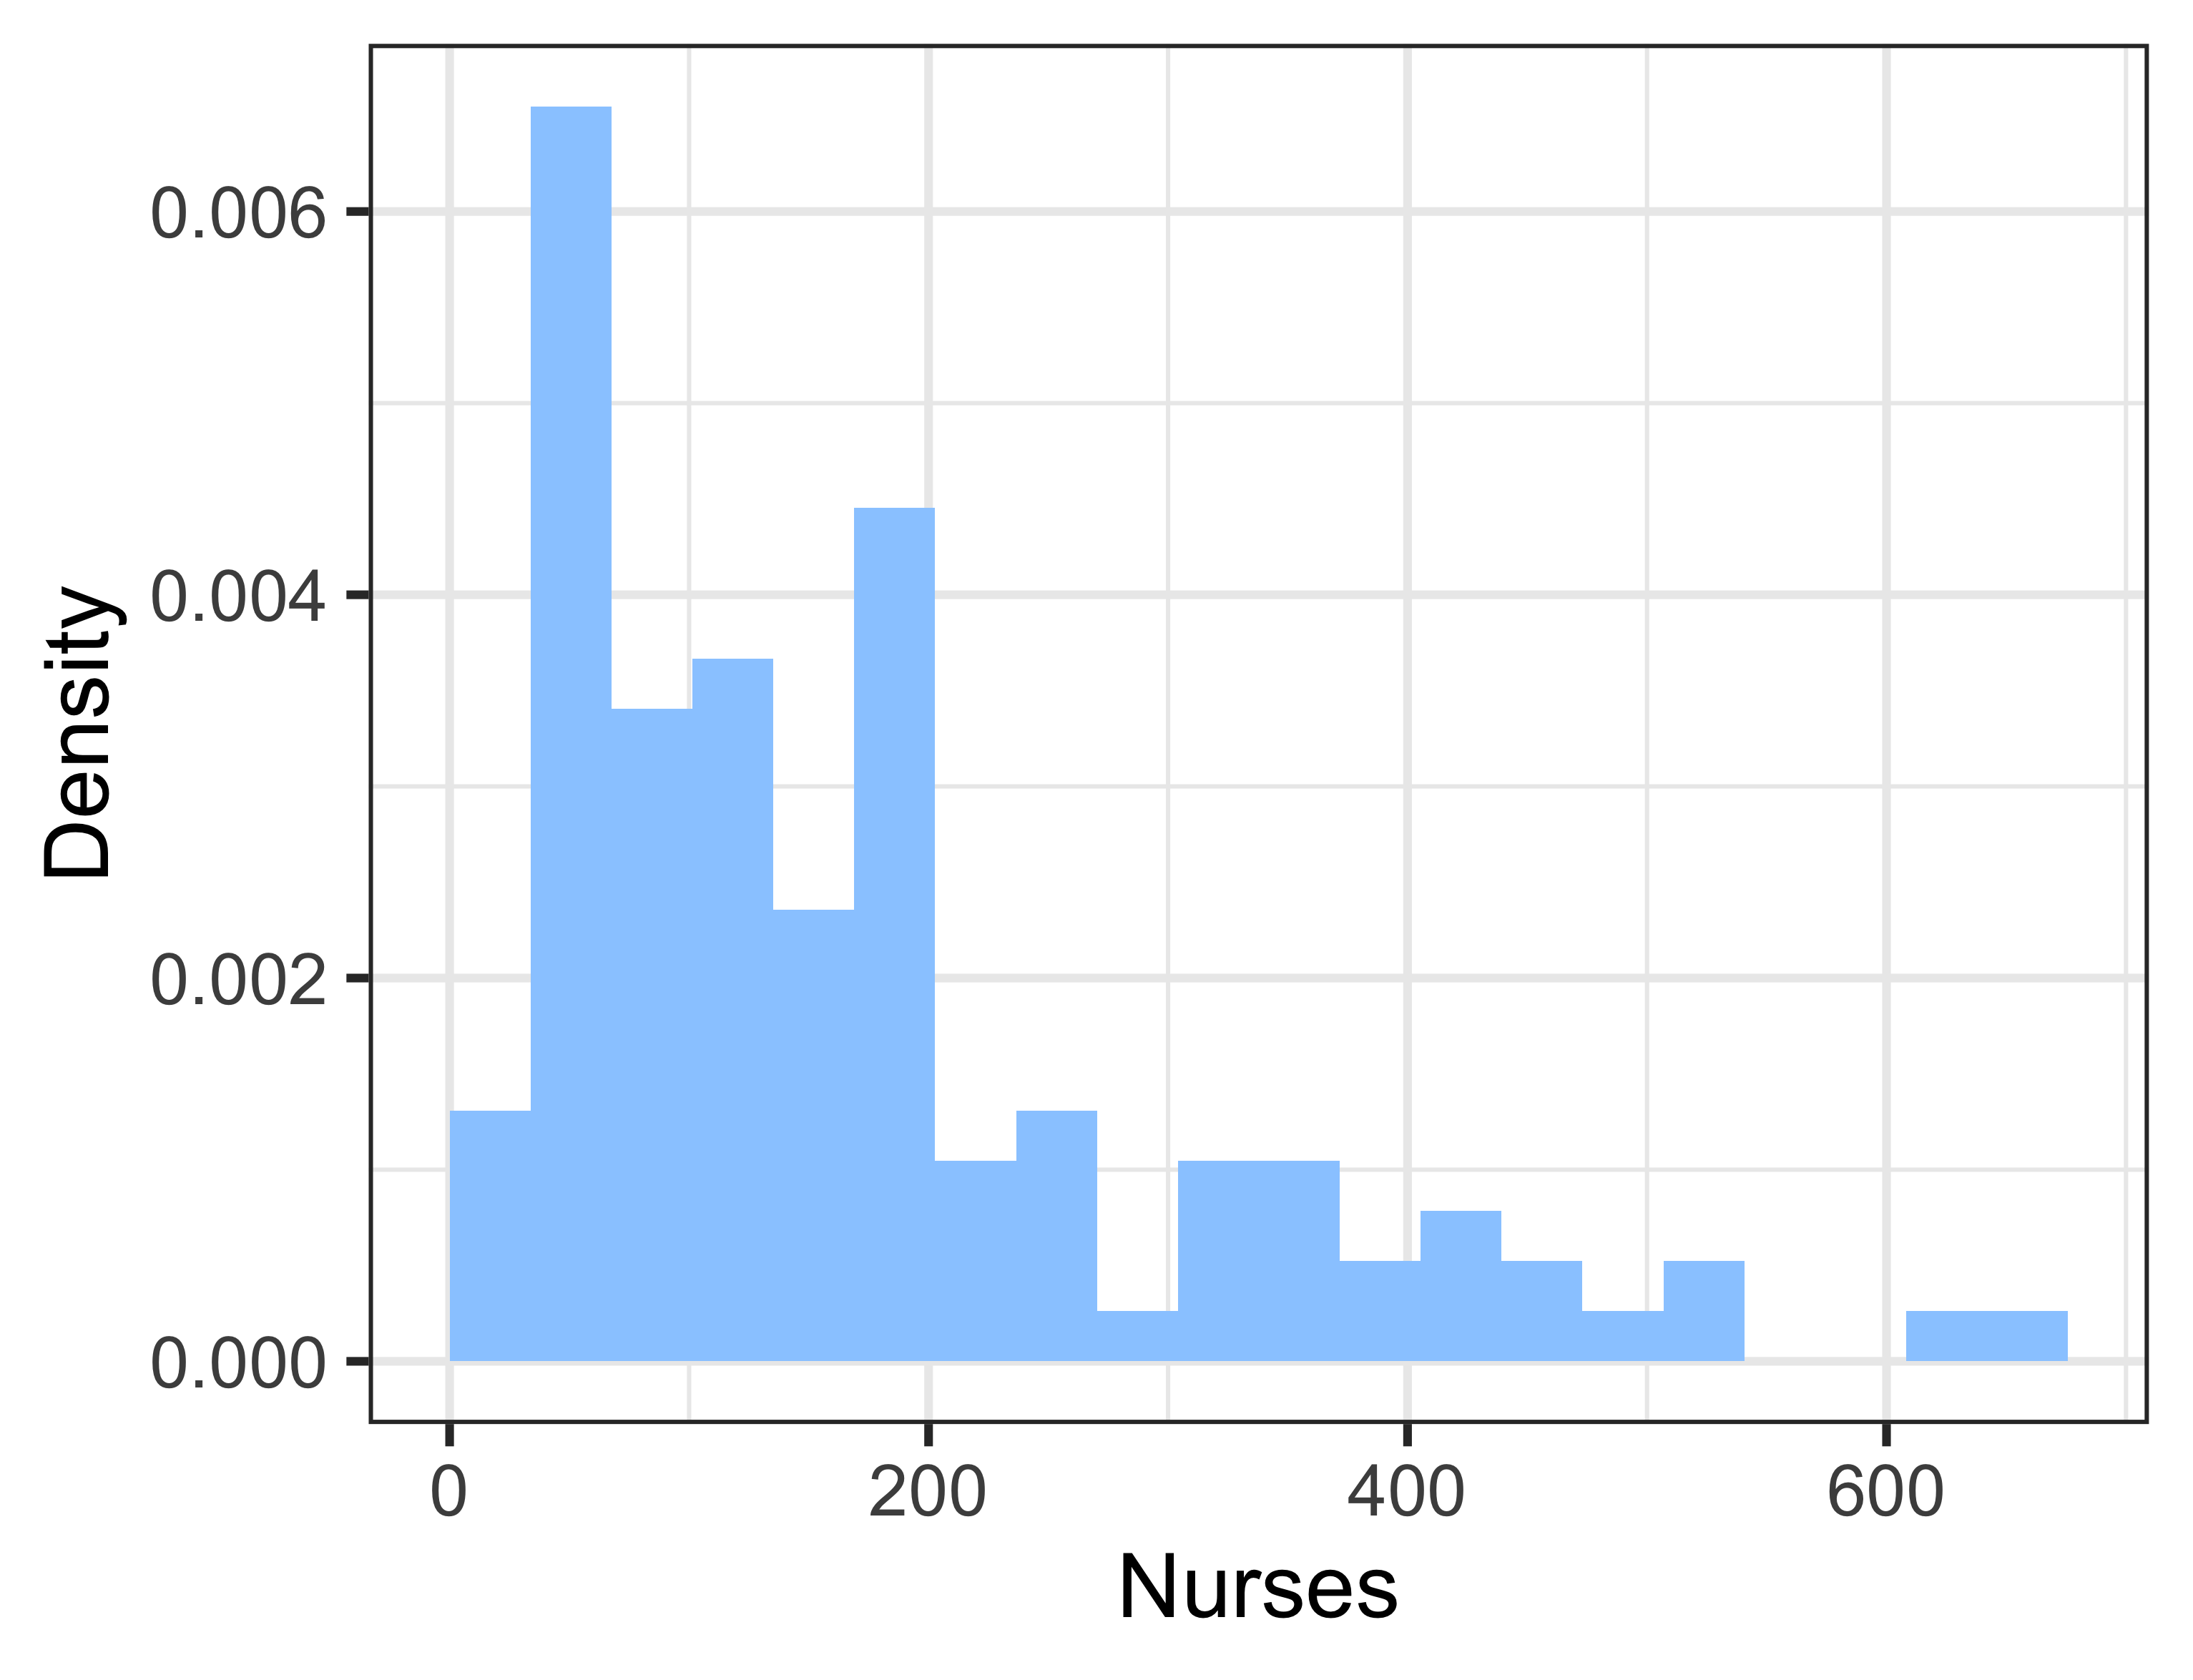
\includegraphics[width = 0.32\textwidth]{img/q01-nurses-hist-original.png}
        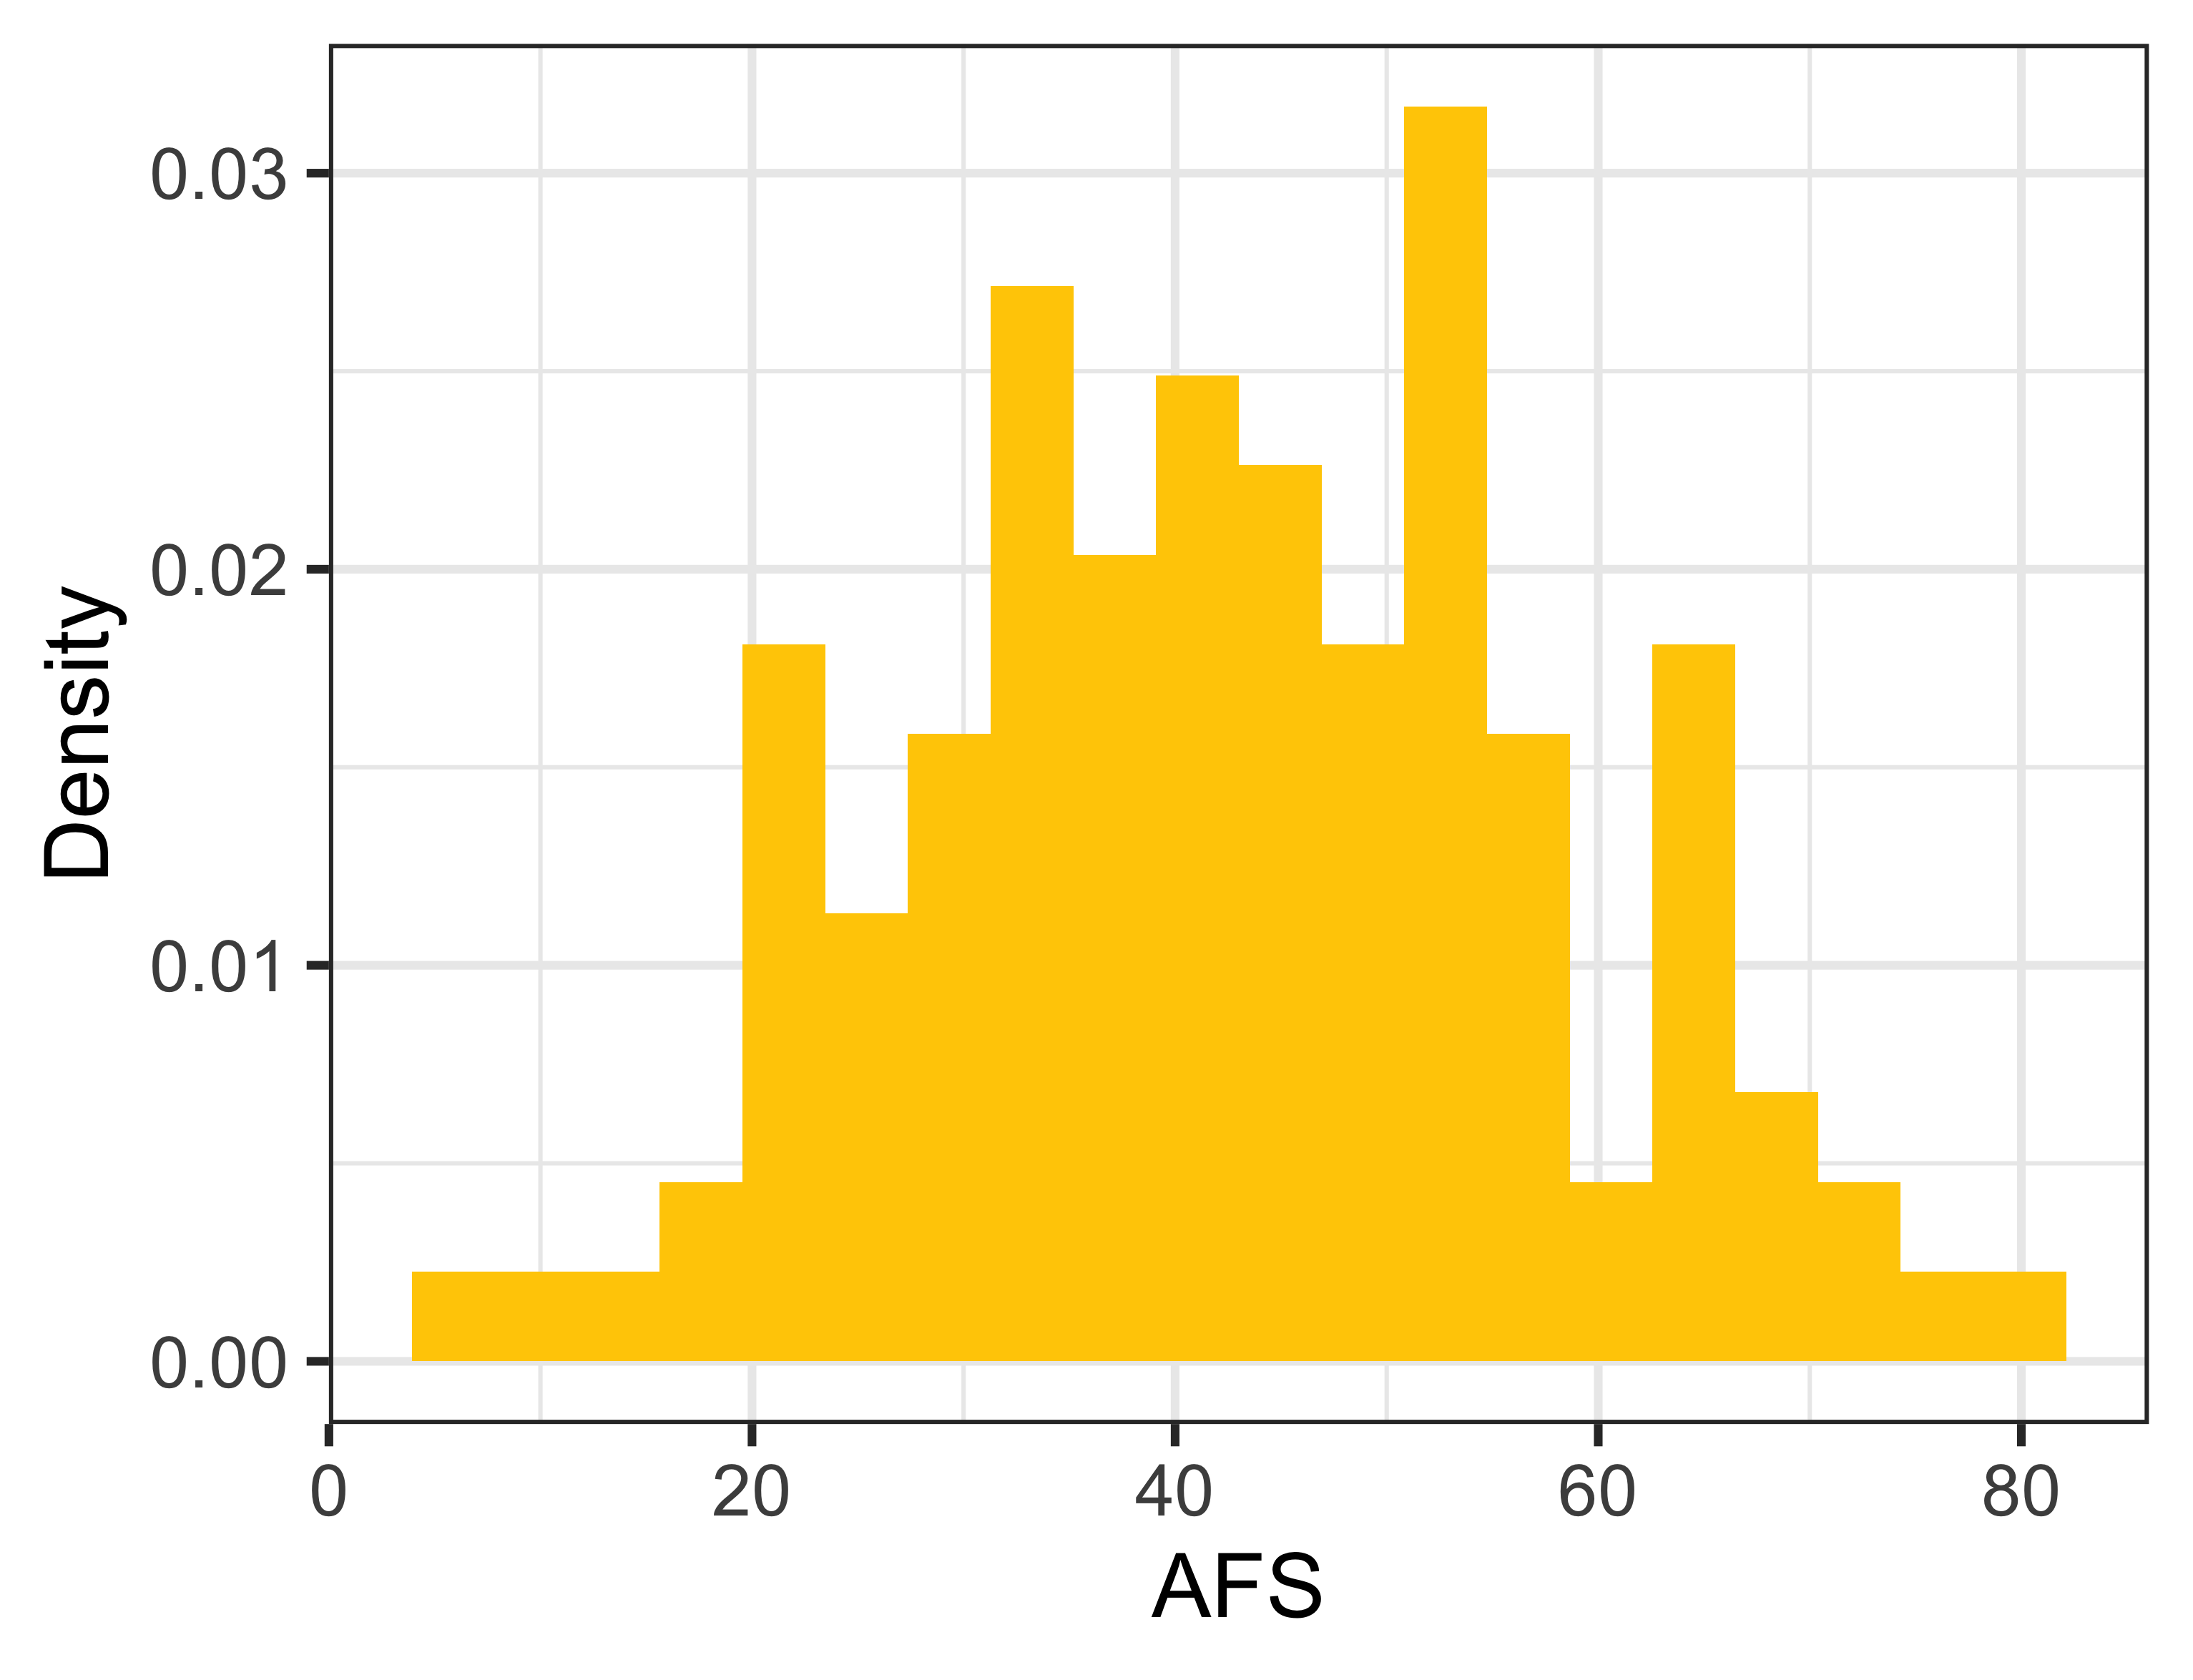
\includegraphics[width = 0.32\textwidth]{img/q01-afs-hist-original.png}
        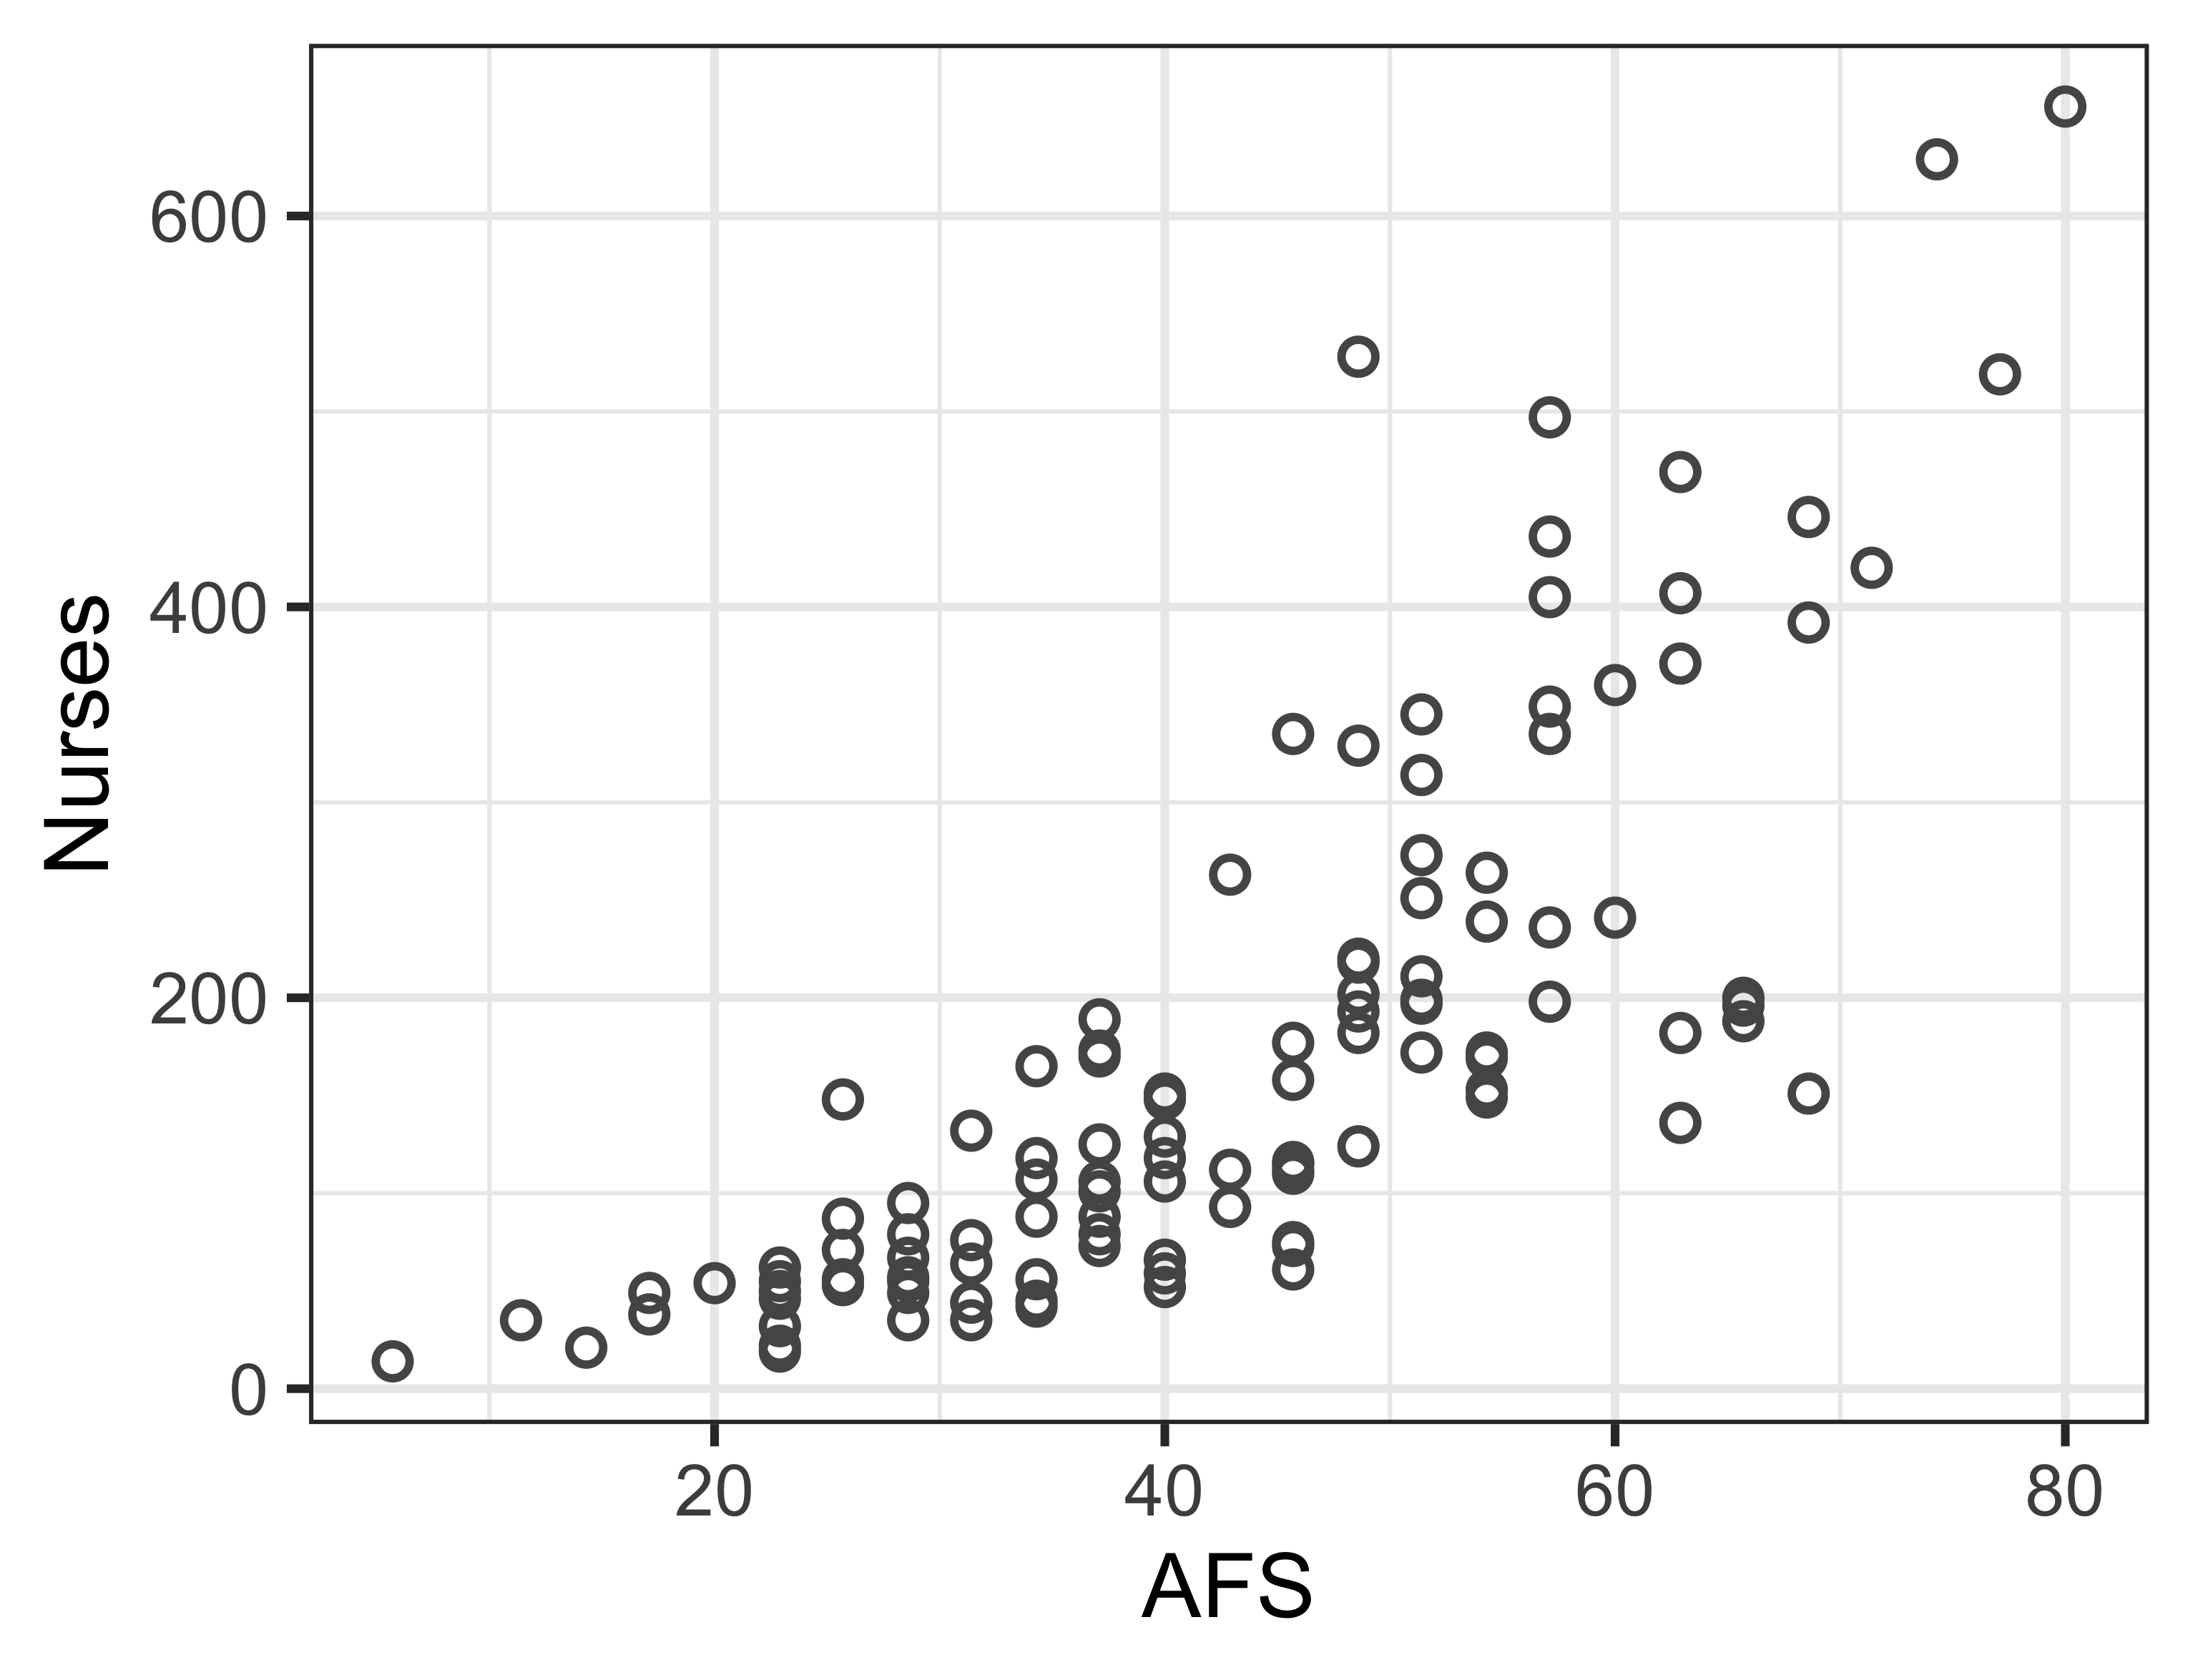
\includegraphics[width = 0.32\textwidth]{img/q01-scatterplot-blank.png}
        \caption{Histograms of \(Y\) and \(X\) and a scatterplot of \(Y\) vs. \(X\).}
        \label{q01-investigation}
    \end{figure}
    \item[(b)] The power transformation function, and its inverse, are defined as 
    \begin{align*}
        g_{\lambda}(Y) 
        = \begin{cases}
            % \frac{Y^{\lambda} - 1}{\lambda} & \text{if } \lambda \neq 0 \\
            (Y^{\lambda} - 1) / \lambda & \text{if } \lambda \neq 0 \\
            \hfil \log Y & \text{if } \lambda = 0.
        \end{cases}
        ~~~\text{and}~~~
        g_{\lambda}^{-1}(Y) 
        = \begin{cases}
            \left( 1 + \lambda Y \right)^{1 / \lambda} & \text{if } \lambda \neq 0 \\
             \hfil \mathrm{exp}(Y) & \text{if } \lambda = 0.
        \end{cases}
    \end{align*}
    Suppose we have our response vector \(\mathbf{y}\) and our observed data \(\mathbf{X}\). 
    We are interested in fitting the model \(\mathbf{g}_{\lambda}(\mathbf{y}) = \mathbf{X}\bm{\beta} + \bm{\epsilon}\), where \(\mathbf{g}_{\lambda}(\mathbf{y})\)
    is the transformed response vector (i.e. the \(i\)th element is given by \(g_{\lambda}(y_i)\)), \(\mathbb{E}[\bm{\epsilon}] = \mathbf{0}\), and 
    \(\mathrm{Var}[\bm{\epsilon}] = \sigma^2 \mathbf{I}\). 
    For notational ease, we will denote \(\mygfull\) as \(\myg\). 
    If we make the further assumption that \(\bm{\epsilon}\) is normally distributed, i.e. 
    \(\bm{\epsilon} \sim \mathrm{N}(\mathbf{0}, \sigma^2 \mathbf{I})\), then our response vector is also normally distributed, where
    \(\myg \sim \mathrm{N}(\mathbf{X}\bm{\beta}, \sigma^2 \mathbf{I})\). It's density function (and thus it's likelihood function) is given by 
    \begin{align*}
        % f(\myg \,|\, \mathbf{X}, \bm{\beta}, \sigma^2, \lambda)
        f(\myg \,|\, \bm{\beta}, \sigma^2, \lambda)
        % f(\myg)
        &= \frac{1}{\sqrt{\mathrm{det}(2 \pi \sigma^2 \mathbf{I})}} \cdot \mathrm{exp} \left( - \frac{(\myg - \mathbf{X}\bm{\beta})^T \big( \sigma^2 \mathbf{I} \big)^{-1} (\myg - \mathbf{X}\bm{\beta})}{2} \right) \\
        &= \frac{1}{(2\pi\sigma^2)^{n/2}} \cdot \mathrm{exp} \left( - \frac{(\myg - \mathbf{X}\bm{\beta})^T (\myg - \mathbf{X}\bm{\beta})}{2 \sigma^2} \right).
    \end{align*}
    Since \(\mathbf{y}\) is a transformation of \(\myg\) (via \(g_{\lambda}^{-1}\)), we can derive the density for \(\mathbf{y}\) as well. Notationally, this result may be somewhat 
    confusing; even though we are finding the density for \(\mathbf{y}\), we will still express the density (partly) in terms of \(\myg\). It is important
    to remember that \(\myg\) is a function of \(\mathbf{y}\). Because the \(i\)th element of \(\myg\) only depends on the \(i\)th element of \(\mathbf{y}\), the Jacobian
    will be a diagonal matrix, and so 
    \begin{align*}
        \mathbf{J}
        = \frac{\partial \myg}{\partial \mathbf{y}}
        = \mathrm{diag} \left( \frac{\partial g_{\lambda}(y_1)}{\partial y_1}, \ldots, \frac{\partial g_{\lambda}(y_n)}{\partial y_n} \right)
        = \mathrm{diag} \big( y_1^{\lambda - 1}, \ldots, y_n^{\lambda - 1} \big), 
    \end{align*}
    and so the density (and thus the likelihood) of \(\mathbf{y}\) is given by 
    \begin{align*}
        g(\mathbf{y} \,|\, \bm{\beta}, \sigma^2, \lambda)
        = f \big( \myg(\mathbf{y}) \big) \cdot \big|\mathrm{det}(\mathbf{J})\big|
        = \frac{1}{(2\pi\sigma^2)^{n/2}} \cdot \mathrm{exp} \left( - \frac{(\myg - \mathbf{X}\bm{\beta})^T (\myg - \mathbf{X}\bm{\beta})}{2 \sigma^2} \right) \cdot \prod_{i=1}^n y_i^{\lambda - 1}.
    \end{align*}
    The log-likelihood \(\ell(\mathbf{y}) = \log g(\mathbf{y})\) is given by 
    \begin{align*}
        \ell(\mathbf{y} \,|\, \bm{\beta}, \sigma^2, \lambda) 
        = - \frac{n}{2} \log (2\pi) - \frac{n}{2} \log (\sigma^2) - \frac{(\myg - \mathbf{X}\bm{\beta})^T (\myg - \mathbf{X}\bm{\beta})}{2 \sigma^2} + (\lambda - 1) \sum_{i=1}^n \log (y_i).
    \end{align*}
    As is standard with maximum likelihood estimation, we now differentiate \(\ell\) with respect to the unknown parameters, set the derivatives to zero, and solve to get the maximum value of \(\ell\). 
    For now, we are going to leave \(\lambda\) fixed and differentiate with respect to \(\bm{\beta}\) and \(\sigma^2\). Doing this for both gives us 
    \(\hat{\bm{\beta}}_{\mathrm{MLE}} = (\mathbf{X}^T\mathbf{X})^{-1}\mathbf{X}^T\myg\) and \(\hat{\sigma}^2_{\mathrm{MLE}} = \myg^T (\mathbf{I} - \mathbf{H}) \myg\), where 
    \(\mathbf{H} = \mathbf{X}(\mathbf{X}^T\mathbf{X})^{-1}\mathbf{X}^T\) is the hat matrix. 
    It is worth noting that both \(\hat{\bm{\beta}}_{\mathrm{MLE}}\) and \(\hat{\sigma}^2_{\mathrm{MLE}}\) are functions of \(\lambda\). 
    Plugging these values back into \(\ell\) will maximize it with respect to \(\bm{\beta}\) and \(\sigma^2\), 
    which means we will only have to maximize it with respect to \(\lambda\). 
    With some simplification, our new loss function is 
    \begin{align*}
        m(\lambda)
        \coloneqq \ell(\mathbf{y} \,|\, \hat{\bm{\beta}}_{\mathrm{MLE}}, \hat{\sigma}^2_{\mathrm{MLE}}, \lambda)
        % \triangleq \ell(\mathbf{y} \,|\, \hat{\bm{\beta}}_{\mathrm{MLE}}, \hat{\sigma}^2_{\mathrm{MLE}}, \lambda)
        % = - \frac{n}{2} \log \left( \frac{2 \pi e}{n} \right) - \frac{n}{2} \log \big( \myg^T(\mathbf{I} - \mathbf{H}) \myg \big) + (\lambda - 1) \sum_{i=1}^n \log(y_i).
        = - \frac{n}{2} \log \left( 2 \pi \mathrm{e} n \right) - \frac{n}{2} \log \big( \myg^T(\mathbf{I} - \mathbf{H}) \myg \big) + (\lambda - 1) \sum_{i=1}^n \log(y_i).
    \end{align*}
    Ideally, we would differentiate \(m\) with respect to \(\lambda\), set \(\partial m / \partial \lambda = 0\), and solve for \(\lambda\). I was unable to 
    derive a closed form solution for the result, but it is still possible to use graphical techniques or numerical methods to find the optimal value of \(\lambda\). 

    We recall that both \(\hat{\bm{\beta}}_{\mathrm{MLE}}\) and \(\hat{\sigma}^2_{\mathrm{MLE}}\) are functions of \(\lambda\), so we cannot know their value until \(\hat{\lambda}_{\mathrm{MLE}}\) has been determined.
    Because of this, as we just showed, the likelihood function can be expressed as a function \(m(\lambda)\) that only depends on \(\lambda\), which can be maximized to find \(\hat{\lambda}_{\mathrm{MLE}}\). 
    Once we find \(\hat{\lambda}_{\mathrm{MLE}}\), we can use this value to determine \(\hat{\bm{\beta}}_{\mathrm{MLE}}\) and \(\hat{\sigma}^2_{\mathrm{MLE}}\). 

    % need to add info about transforming model back to y, here and in paragraph below
    % maybe put into appendix?

    The left panel of Figure \ref{q01-box-cox} shows a plot of \(m(\lambda)\) against \(\lambda\) for values \(\lambda \in [-1, 1]\). The log-likelihood is maximized when \(\hat{\lambda}_{\mathrm{MLE}} = 0.09\).
    The middle panel shows the histogram of \(g_{0.09}(Y)\), the transformed version of \(Y\), and we can see with this value of \(\lambda\) that \(\myg\) is normally distributed. 
    We can now 
    \begin{figure}
        \centering
        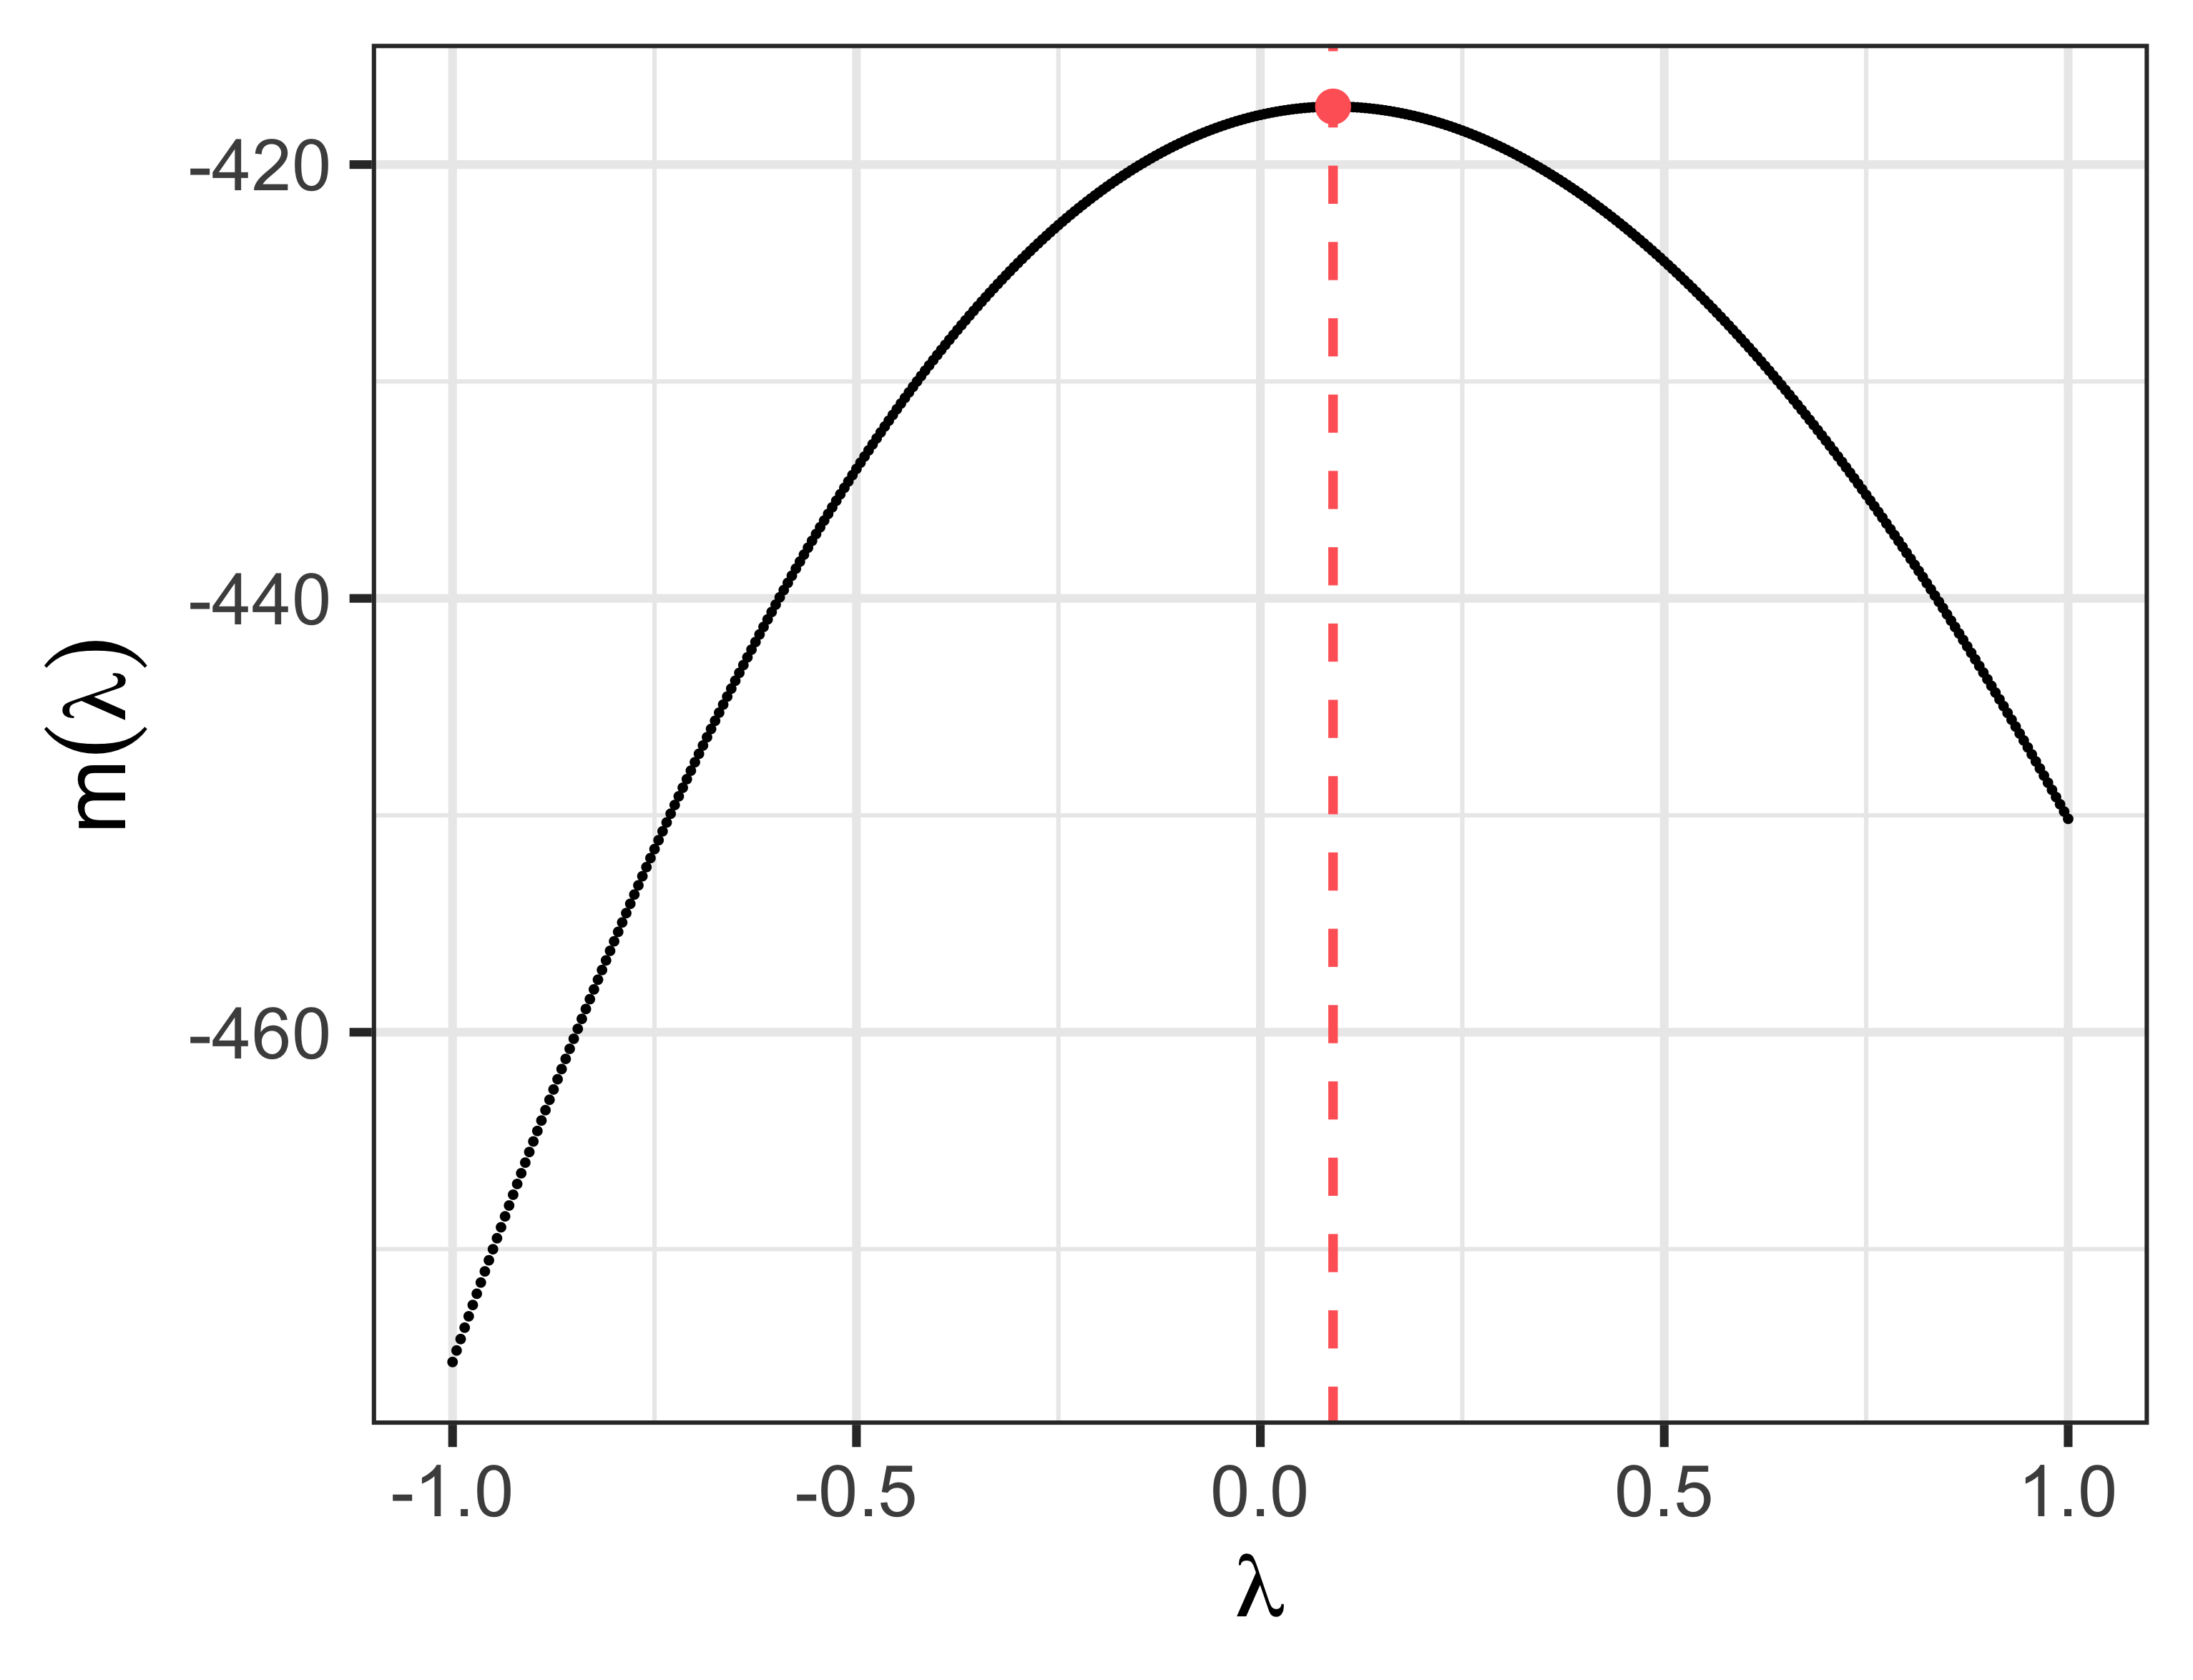
\includegraphics[width = 0.32\textwidth]{img/q01-box-cox-lambda.png}
        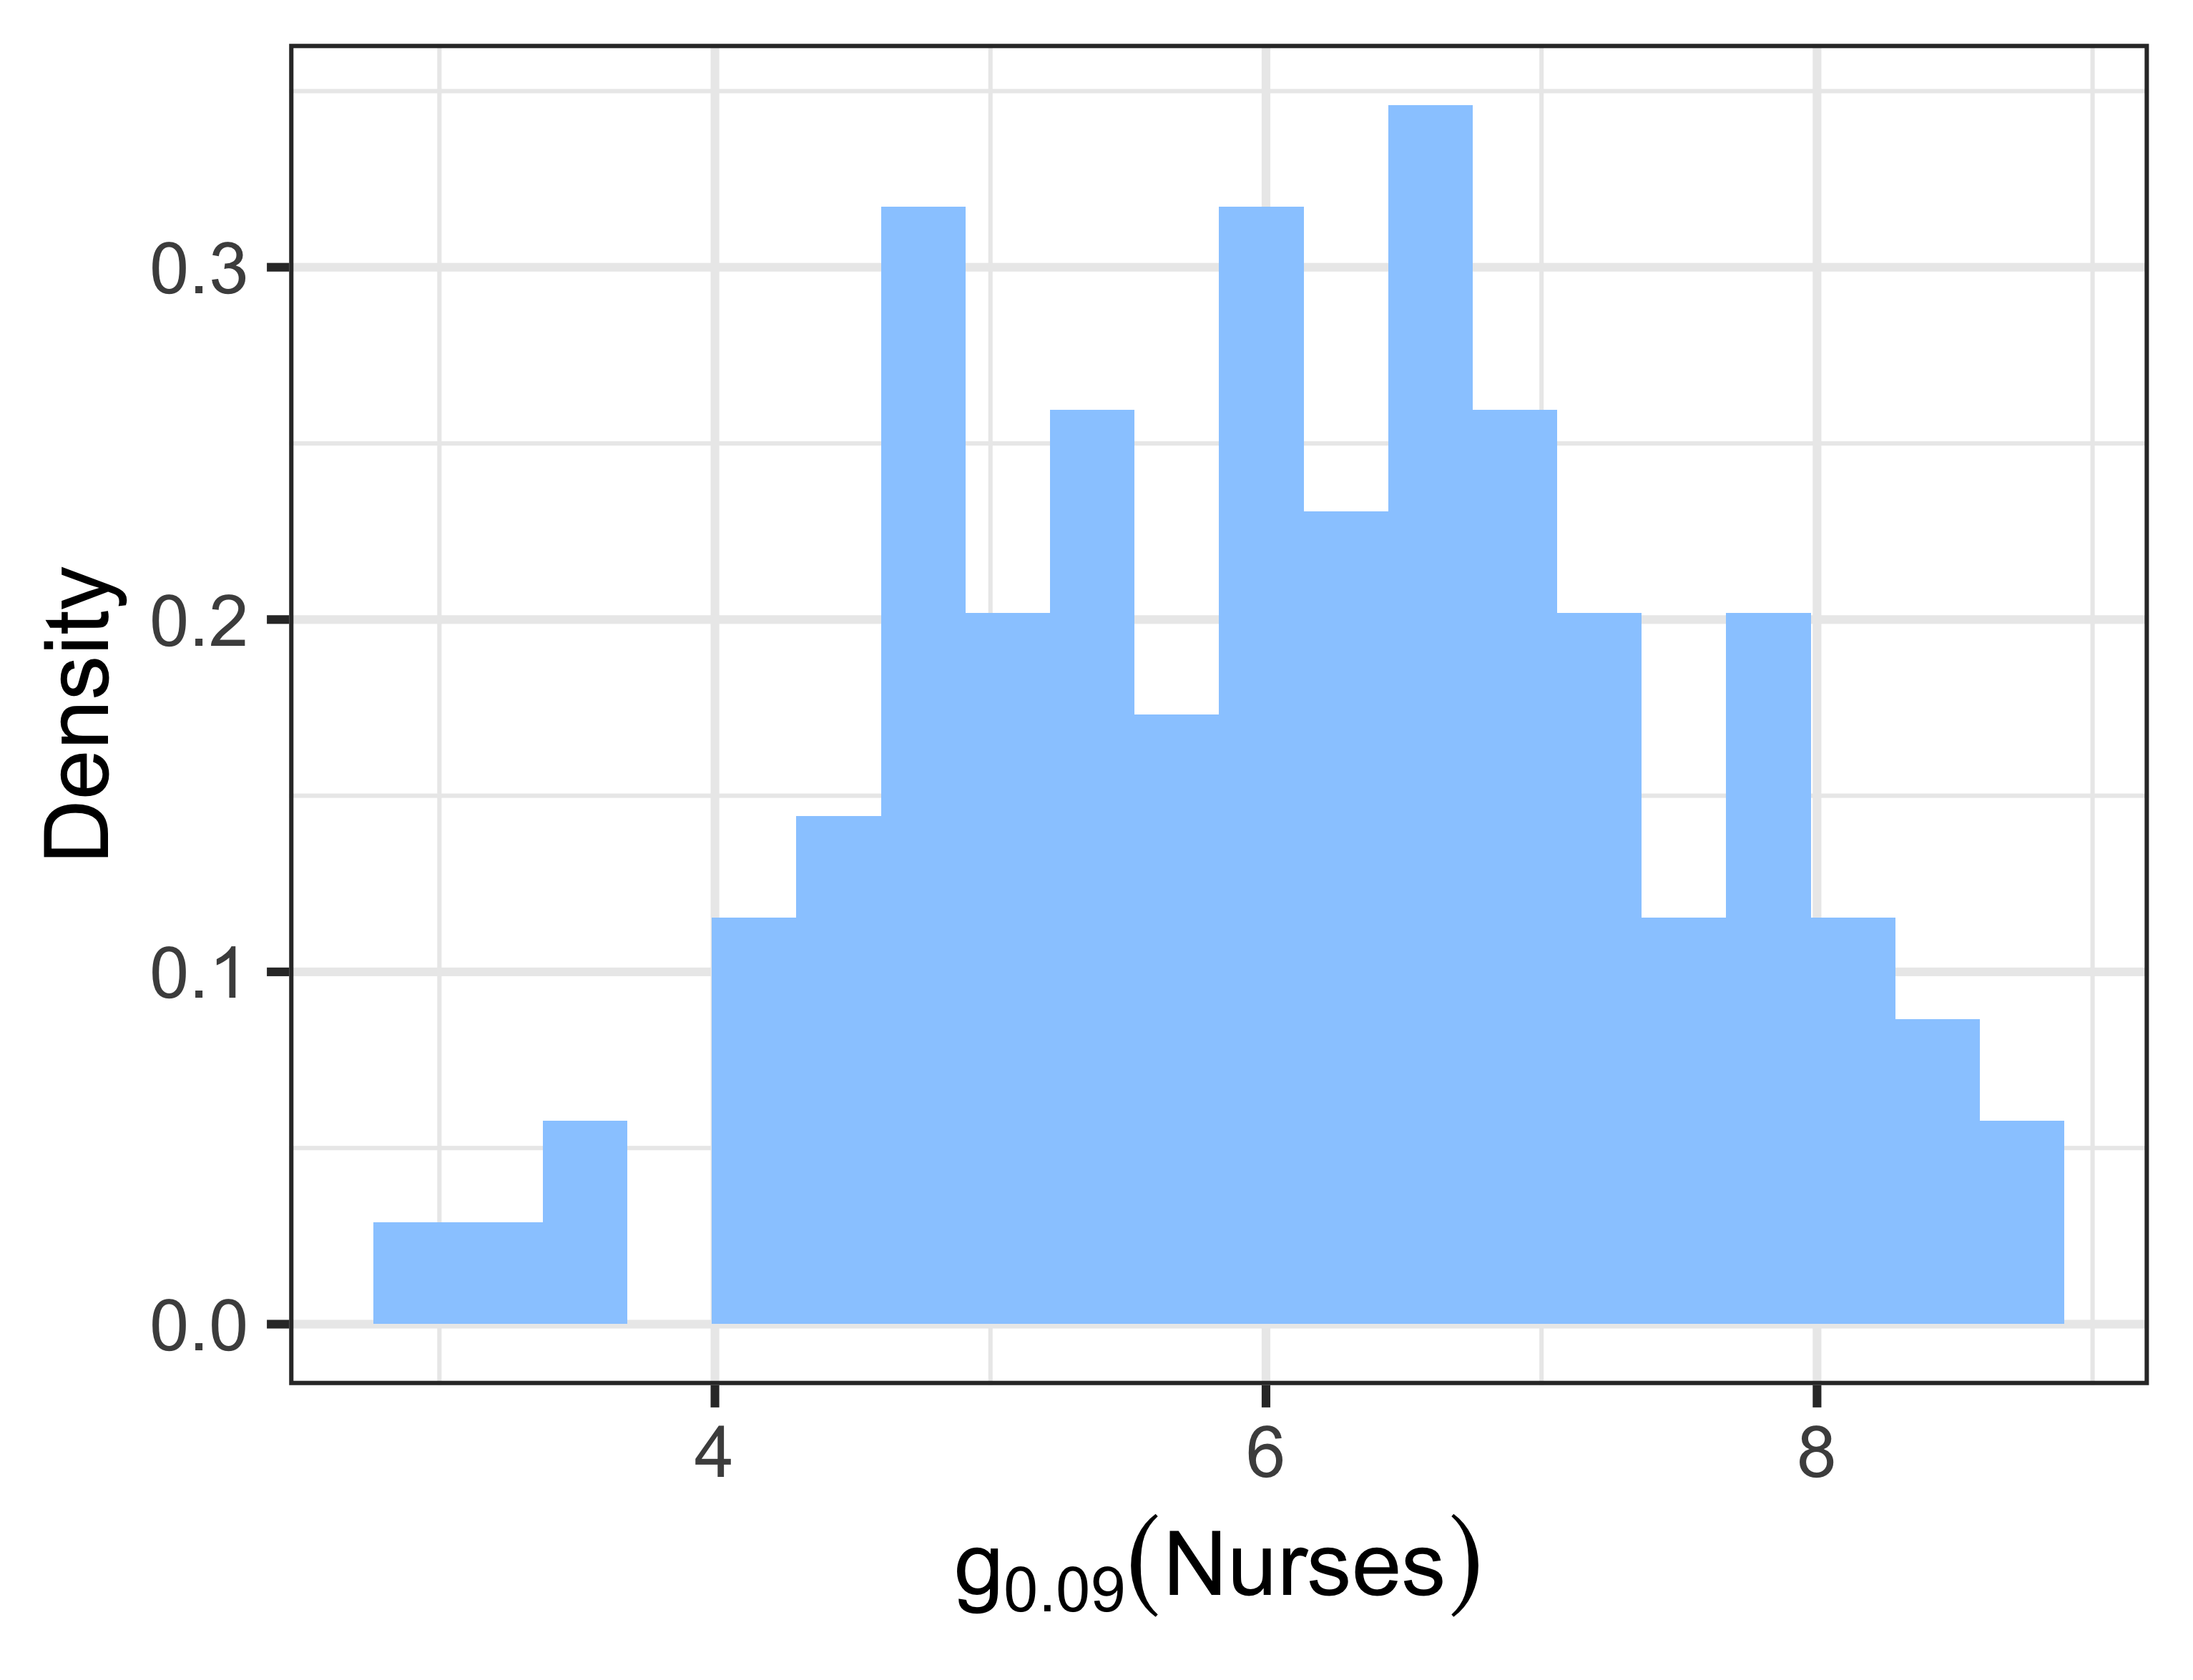
\includegraphics[width = 0.32\textwidth]{img/q01-nurses-hist-transformed.png}
        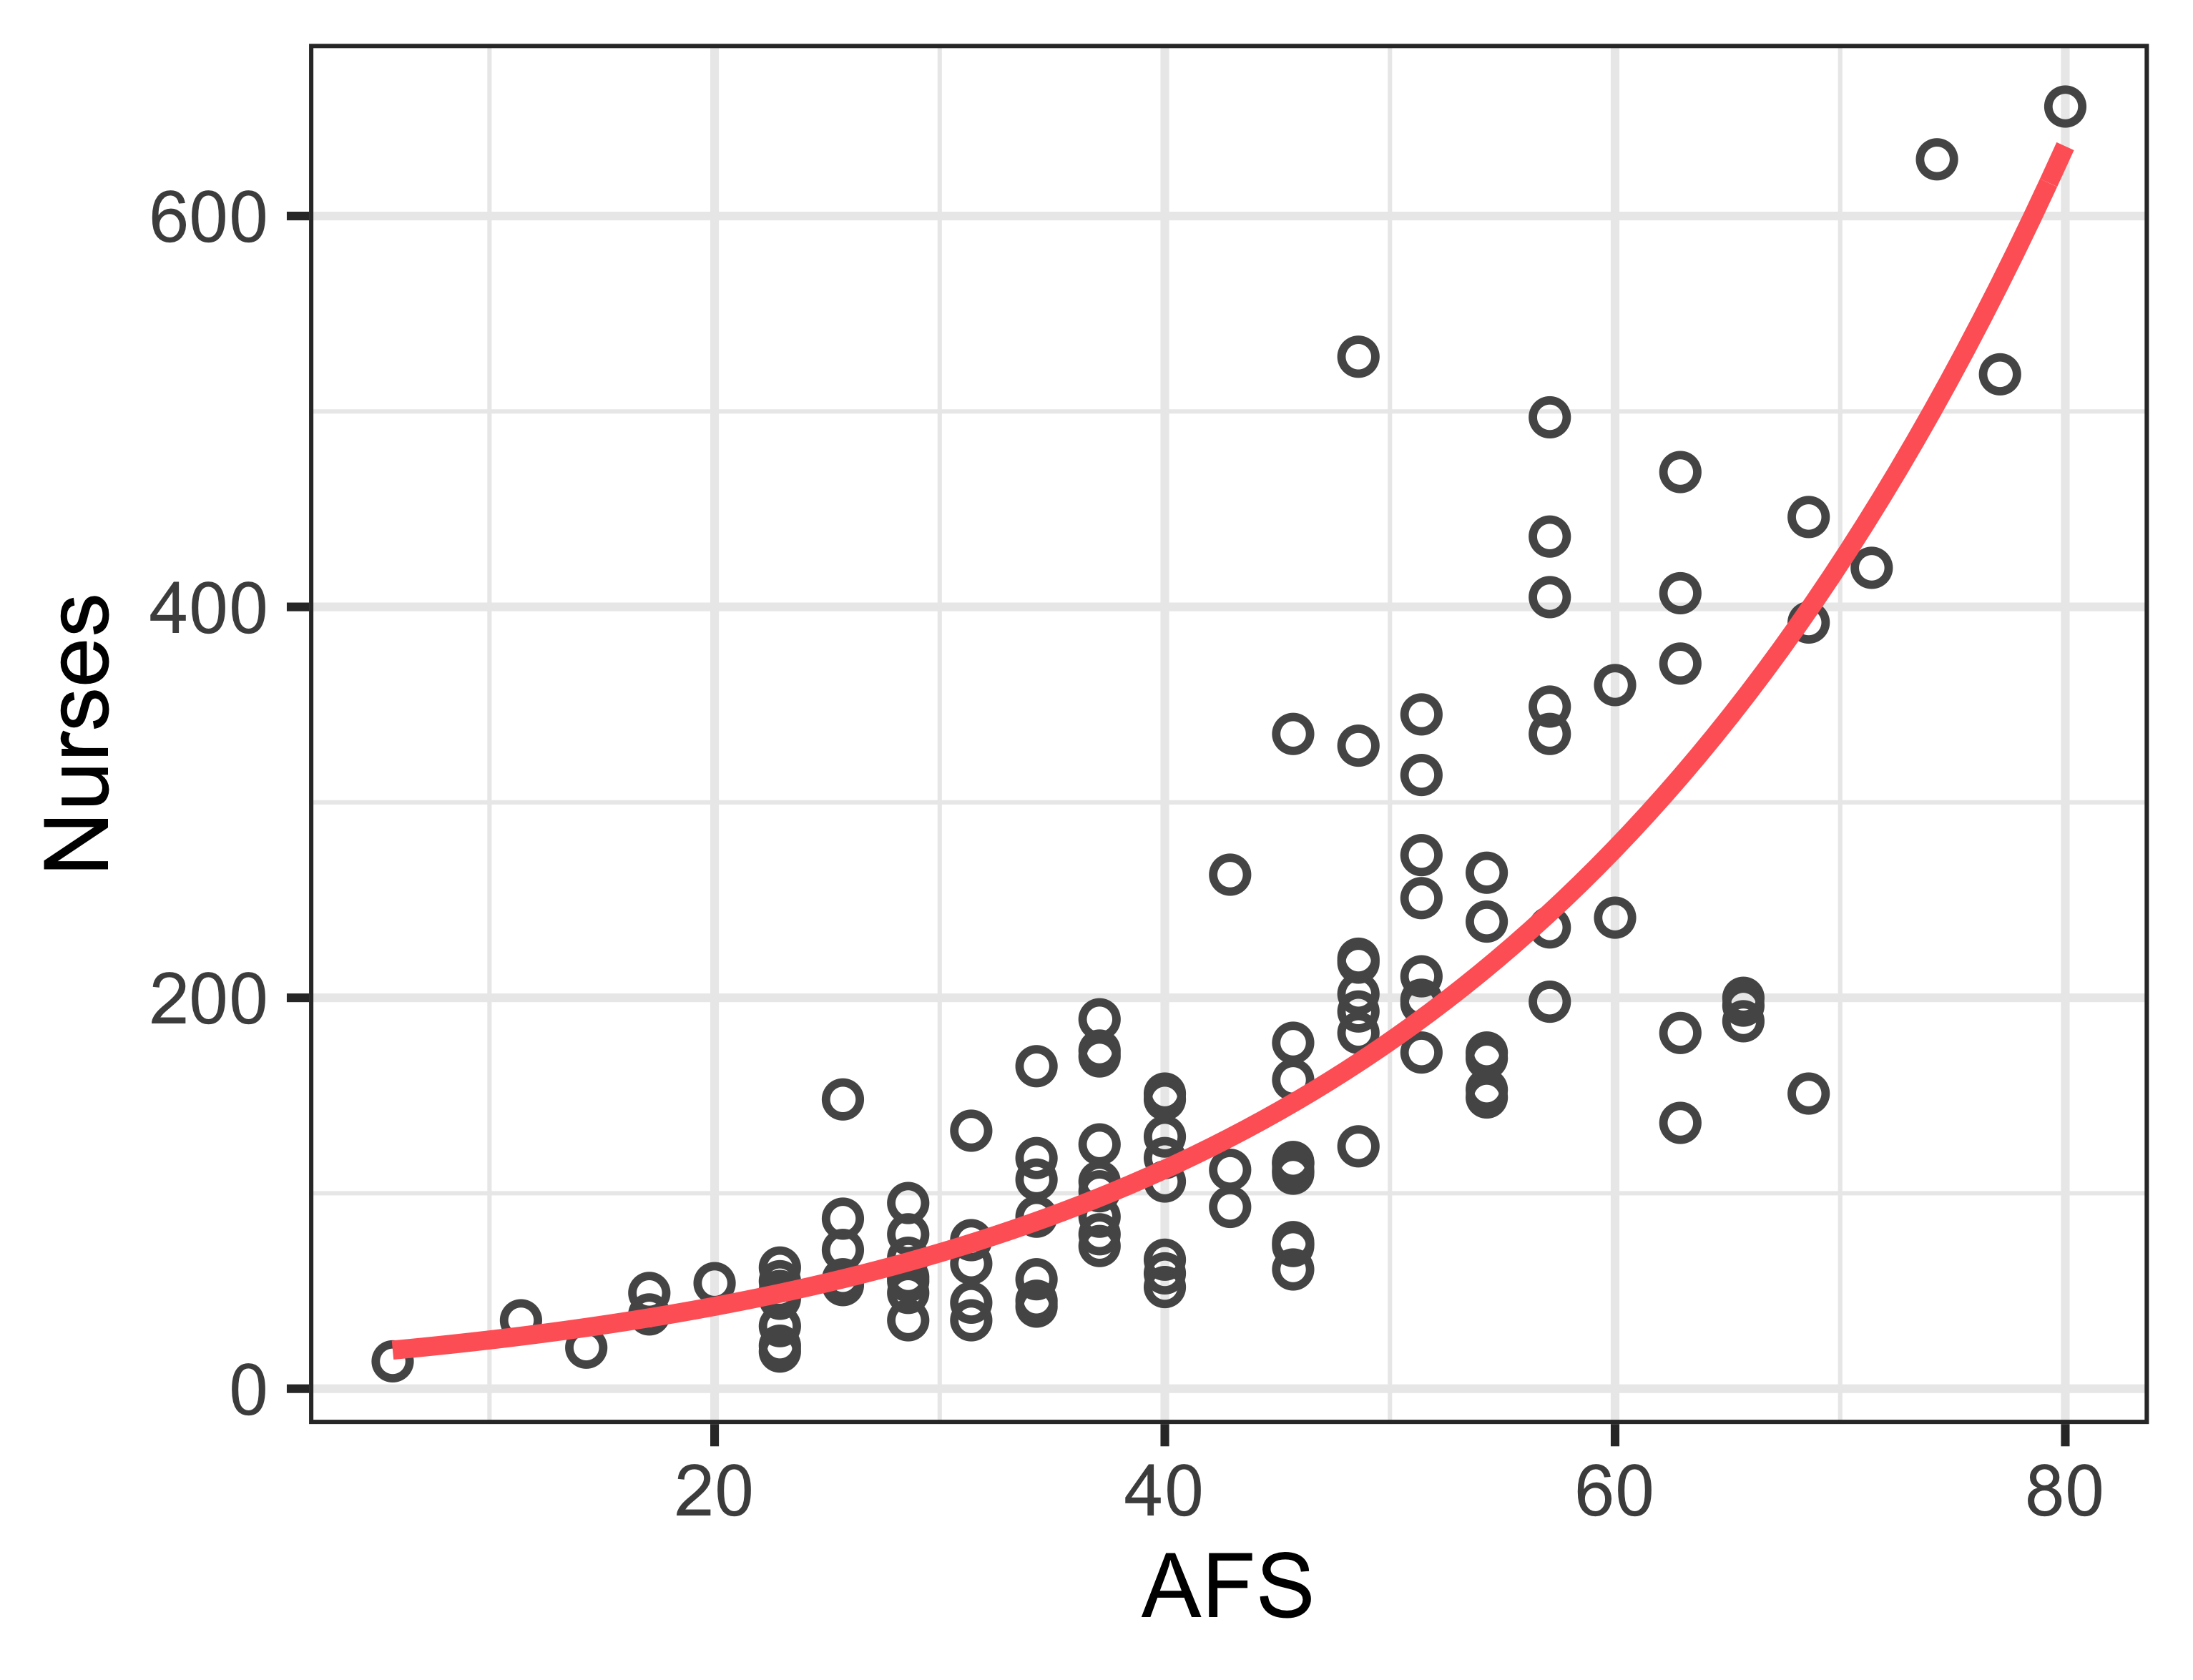
\includegraphics[width = 0.32\textwidth]{img/q01-scatterplot-model.png}
        \caption{Relevant plots for the Box-Cox transformation of \(Y\).}
        \label{q01-box-cox}
    \end{figure}

    \item[(c)] 
\end{itemize}

\end{document}